\chapter[Modellierung als Computerprogramm]{Modellierung von Patchwork als Computerprogramm}
\label{chapter:modellierung-von-patchwork-als-computerprogramm}

Ein wesentlicher Schritt in der Entwicklung von Computerspielengines besteht in der Modellierung und Umsetzung des Spiels als Computerprogramm. Da Engines in der Regel darauf basieren mehrere zehntausende von Aktionen vorrausschauen \cite{2018.AlphaZero}, muss die zugrundeliegende Implementierung so effizient wie möglich sein. Eine erste prototypische Implementierung von Patchwork in Python führte zu Zuggenerierungszeiten von ca. $100\acs{ms}$, was in 10 Sekunden aber gerade mal die Analyse von 100 möglichen Zügen bedeutet. Aus diesem Grund wird Patchwork mit der Programmiersprache \emph{Rust} \cite{2014.Rust} umgesetzt. Rust hat Performance als ein Hauptziel und zeichnet sich durch eine schnelle und speichereffiziente Ausführung aus \cite{2024.Rust}. Zusammen mit weiteren Effizienzoptimierungen führt dies zu Ausführungszeiten im Mirkosekundenbereich (Tabelle \ref{tabelle:patchwork-methods}).

\lstinputlisting[
    label={code:patchwork-state},
    caption={Patchwork-Zustand},
    captionpos=b,
    language=Rust,
    firstline=0,
]{res/code/patchwork-state.rs}

Der gesamte Zustand von Patchwork wird zu jeder Zeit durch die in Codeausschnitt \ref{code:patchwork-state} dargestellte Struktur \code{Patchwork} repräsentiert. Alle noch verfügbaren Flicken werden in \code{patches} in der Reihenfolge gespeichert, wie sie vor der Spielfigur liegen. Der \code{turn\_type} zeigt an, ob es sich bei den derzeit verfügbaren Aktionen um eine normale Aktion handelt oder ob ein Spezialflicken gelegt werden muss. Der derzeitige Spieler, der Inhaber des $7\times 7$ Sonderplättchens und der Spieler, welcher als erstes das Ziel erreicht hat, werden im Bitfeld \code{status\_flags} festgehalten, sofern vorhanden. Letzteres ist relevant, um bei einem beendeten Spiel mit gleicher Punktzahl den Gewinner identifizieren zu können.

Der Zeitplan wird mittels der \code{TimeBoard}-Struktur modelliert. Diese hält intern nur ein einfache \ac{u8}-Array der Länge 54. Bei jedem Eintrag des Arrays handelt es sich wiederrum um ein Bitfeld. Dieses kann signalisieren, ob sich Spieler 1 und 2, ein Knopfeinkommen oder ein Spezialflicken auf ihrem Feld befindet. Knopfeinkommen und Spezialflicken befinden sich im originalen Spiel zwischen 2 Feldern. Im Array werden sie einfach in dem Feld nach ihrer Originalposition gespeichert. Sobald solch ein Feld von einem Spieler erreich wird, tritt der Effekt ein, was zu gleichem Verhalten wie im Brettspiel führt.

Zuletzt existiert für jeden Spieler noch ein Zustand in der Patchwork-Struktur. Der Zustand jeden Spielers setzt sich dabei aus 3 Komponenten zusammen. Zuerst wird hier auch die Position des Spielers gespeichert, um Zugriff in konstanter Zeit zu ermöglichen. Weiterhin wird der derzeitig verfügbare Knopfvorrat des Spielers gespeichert. Zuletzt wird noch auf eine weitere Struktur, das \code{QuiltBoard}, verwiesen.

\section{Aufbau des Ablageplans}

\lstinputlisting[
    label={code:quilt-board-definition},
    caption={Definition der QuiltBoard-Struktur},
    captionpos=b,
    language=Rust,
    firstline=0,
]{res/code/quilt-board-definition.rs}
\vspace*{-0.3cm}

Die in Codeausschnitt \ref{code:quilt-board-definition} definierte Struktur \code{QuiltBoard} modelliert den Ablageplan eines Spielers. Dabei existieren nur 2 Attribute. Zuerst wird das Knopfeinkommen mit \code{button\_income} gespeichert, was durch die auf dem Ablageplan liegenden Flicken beim Passieren einer Knopf-Wertung generiert wird. Das zweite Attribut \code{tiles} dient dazu, den Status der einzelnen Felder auf dem Ablageplan zu speichern. Der Ablageplan besteht aus 81 Feldern, die in 9 Zeilen und 9 Spalten angeordnet sind, und für die jeweils gespeichert werden muss, ob das Feld belegt ist oder nicht. Da alle Abfragen bezüglich Status der Felder so schnell wie möglich sein sollen, kommt hier anstatt eines üblichen 2-dimensionalen Arrays eine \ac{u128} zum Einsatz. Da nur zwei Zustände existieren, kann für jedes Feld ein Bit verwendet werden. Weiterhin werden alle Felder des Ablageplans zeilenweise wie in Abbildung \ref{fig:quilt-board-storage} in einer Ganzzahl nacheinander abgelegt.

\vspace*{-5cm}
\pagebreak

\begin{figure}[!ht]
    \centering
    \rlap{{\color{white}\acf{LSB} \acf{MSB}}} \vspace*{-\baselineskip}
    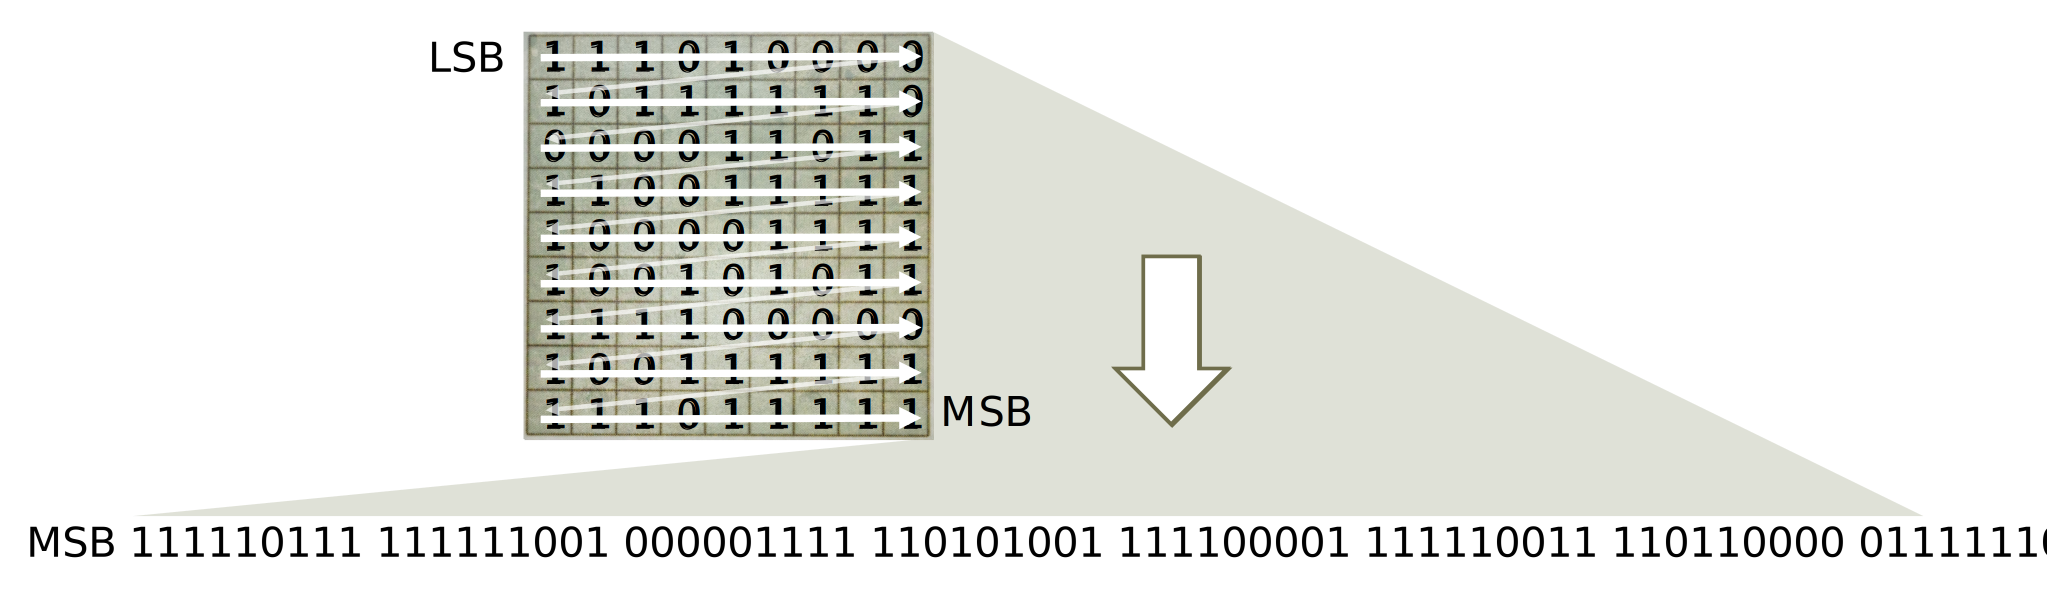
\includegraphics[width=\textwidth]{res/pictures/quilt-board-storage.pdf}
    \caption{Zeilenweise Anordnung der Felder des Ablageplans}
    \label{fig:quilt-board-storage}
\end{figure}

Da der Ablageplan 81 Felder umfasst, muss $2^7=128$ Bit als Ganzzahldatentyp verwendet werden. Dieser wird von Rust nativ unterstützt und für 64 Bit Rechner in mehrere Operationen kompiliert. Die oberen Bits der Zahl sind dabei immer auf 0 gesetzt. Durch die effiziente Speicherung des Ablageplans in einem \ac{u128}, können Abfragen bezüglich Befüllung oder Überlagerung von Feldern in konstanter Zeit durch Bitmasken und Bitoperationen durchgeführt werden. Als Beispiel lässt sich hier die Methode zum Überprüfen der notwendigen Bedingung zur Erhaltung des $7\times 7$ Sonderplättchen anführen (Anhang \ref{code:quilt-board-special-tile-condition}).

Besonders anzumerken ist, dass die Flicken und ihre Transformationen, wie sie auf dem Ablageplan liegen, nicht gespeichert werden. Da einige Computergegner wie beispielsweise der \ac{MCTS}-Spieler den Spielstand sehr oft kopieren müssen und die genaue Position der Flicken für die Generierung und Ausführung von Aktionen nicht benötigt wird, würde diese Extrainformation nur zu unnötig erhöhtem Speicherverbrauch führen.

\section{Modellierung der Aktionen}

TODO: Action, ActionId/SurrogateActionId, NaturalActionId

\begin{itemize}
    \item \code{Action} als Tagged-Union
    \item \code{ActionId} bzw. \code{SurrogateActionId} als \ac{u32}
    \item \code{NaturalActionId} als TODO: 2028
\end{itemize}

TODO:

\lstinputlisting[
    label={code:action},
    caption={Definition des Tagged-Union \code{Action}},
    captionpos=b,
    language=Rust,
    firstline=0,
]{res/code/action.rs}

\section{Flicken und Zugmöglichkeiten}

\acs{u128}

\pagebreak

\begin{table}[H]
    \centering
    \resizebox{\textwidth}{!}{\begin{tabular}{|l|r|c|l|}
            \hline
            \multicolumn{1}{|c|}{Methode}                                                 & \multicolumn{1}{|c|}{Zeit}      & $\mathcal{O}$-Kalkül        & \multicolumn{1}{|c|}{Bemerkungen}                  \\ \hline
            \code{game.get\_initial\_state}                                               & $472{,}11\,\acs{ns}$            & $\mathcal{O}\left(n\right)$ & $n$ aufgrund Mischen der Flicken                   \\  \hline
            \code{game.get\_valid\_actions}                                               & $8{,}91\,\acs{us}$              & $\mathcal{O}\left(n\right)$ & $3\times$Aufruf von Ablageplan Aktionen generieren \\  \hline
            \code{game.get\_random\_action}                                               & $9{,}22\,\acs{us}$              & $\mathcal{O}\left(n\right)$ & Aufruf von \code{get\_valid\_actions}              \\  \hline
            \code{game.do\_action}                                                        & $280{,}00\,\acs{ns}$            & $\mathcal{O}\left(1\right)$ &                                                    \\  \hline
            \code{game.undo\_action}                                                      & $286{,}78\,\acs{ns}$            & $\mathcal{O}\left(1\right)$ &                                                    \\  \hline
            \code{game.clone}                                                             & $1{,}36\,\acs{us}$              & $\mathcal{O}\left(1\right)$ & $\hat{=}$ \code{memcpy}                            \\  \hline
            \code{game.is\_terminated}                                                    & $84{,}79\,\acs{ns}$             & $\mathcal{O}\left(1\right)$ &                                                    \\  \hline
            {\footnotesize \code{action\_id.from\_natural\_action\_id} }                  & $42{,}44\,\acs{ns}$             & $\mathcal{O}\left(1\right)$ &                                                    \\  \hline
            {\footnotesize \code{natural\_action\_id.from\_surrogate\_action\_id} }       & $45{,}97\,\acs{ns}$             & $\mathcal{O}\left(1\right)$ &                                                    \\  \hline
            \code{patch\_manager.get\_patch}                                              & $1{,}87\,\acs{ns}$              & $\mathcal{O}\left(1\right)$ &                                                    \\  \hline
            \code{patch\_manager.get\_special\_patch}                                     & $3{,}70\,\acs{ns}$              & $\mathcal{O}\left(1\right)$ &                                                    \\  \hline
            \code{patch\_manager.get\_transformation}                                     & $2{,}57\,\acs{ns}$              & $\mathcal{O}\left(1\right)$ &                                                    \\  \hline
            \code{player.get\_position}                                                   & $41{,}93\,\acs{ns}$             & $\mathcal{O}\left(1\right)$ &                                                    \\  \hline
            \code{quilt\_board.is\_full}                                                  & $561{,}16\,\acs{ps}$            & $\mathcal{O}\left(1\right)$ &                                                    \\  \hline
            {\footnotesize \code{quilt\_board.is\_special\_tile\_condition\_reached} }    & $523{,}76\,\acs{ps}$            & $\mathcal{O}\left(1\right)$ &                                                    \\  \hline
            \code{quilt\_board.do\_action}                                                & $46{,}90\,\acs{ns}$             & $\mathcal{O}\left(1\right)$ &                                                    \\  \hline
            \code{quilt\_board.undo\_action}                                              & $47{,}18\,\acs{ns}$             & $\mathcal{O}\left(1\right)$ &                                                    \\  \hline
            {\footnotesize \code{quilt\_board.get\_valid\_actions\_for\_patch} }          & $1{,}27\,\acs{us}$              & $\mathcal{O}\left(n\right)$ &                                                    \\  \hline
            {\footnotesize \code{quilt\_board.get\_valid\_actions\_for\_special\_patch} } & $855{,}98\,\acs{ns}$            & $\mathcal{O}\left(n\right)$ &                                                    \\  \hline
            Getter\textendash{} und Setter\textendash{}Methoden                           & \multicolumn{1}{|c|}{$\diagup$} & $\mathcal{O}\left(1\right)$ &                                                    \\  \hline
        \end{tabular}}
    \vspace{3pt}
    \caption{Übersicht über die verfügbaren Methoden in der Patchwork\textendash{}Implementierung}
    \label{tabelle:patchwork-methods}
\end{table}

TODO: Hier fehlt noch der Anhang + Verweis für Benchmark

\begin{itemize}
    \item Aufbau des Spielfeldes
    \item Speicherung der Quilt Boards (Row-Major)
    \item Speicherung des Time Boards
    \item Speicherung der Patchliste
    \item Umsetzung von Zügen
    \item Effizienzoptimierungen (u128, vorberechnete Transformationen, ...)
    \item Abstraction von Player Interface
    \item Evaluator, Move Orderer, Tree Policy (wahrscheinlich später)
\end{itemize}
